\chapter{Introduction}
The ability to communicate with the user in a natural language is a major driving
force in development of natural language processing algorithms. One of the basic
tasks in a NLP pipeline is parsing by which we can describe sentence structure.
There exist two basic parsing techniques: constituency and dependency parsing.
With constituency parser we break the sentence into phrases, which can be furher
broken into smaller sub-phrases. Example of such parsing is shown in figure
\ref{fig:constituency_tree}.

\begin{figure}[!htbp]
  \centering
  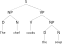
\includegraphics[width=0.4\linewidth]{img/examples/dep/constituent.png}
  \caption{A sample constituency parse tree\todotext{ściągnięte z internetu, przegenerować wektorowo}} 
  \label{fig:constituency_tree}
\end{figure}

In dependency parsing each word (called \emph{dependent})
is connected via labelled arc to another word of the sentence (called \emph{head})
or to the special \emph{ROOT} vertice, forming a directed tree.
Example of such parsing is depicted on figure \ref{fig:dependency_tree}.

\begin{figure}[!htbp]
  \centering
  \resizebox{0.8\textwidth}{!}{
    \import{img/examples/dep/}{dep.pdf_tex}
  }
  \caption{A sample dependency parse tree} 
  \label{fig:dependency_tree}
\end{figure}

A major advantage of dependency parsers over constituency ones are their
independence from the word ordering. It is important in morphologically rich
languages like Polish or Czech where the ordering is very flexible, and thus
related words can be far apart from each other.
Additionaly the head-dependent relationship is a good approximation to semantic
relationship between words \cite{covington_fundamental_2001} which is important
for tasks like question answering or information extraction.

The labels of head-dependent arcs tells us about grammatical function that
dependent word have in respect to the head. In table \ref{tab:label_samples}
we show some of the most popular labels for the english language.

\begin{table}[!htbp]
    \centering
    \begin{tabular}{c | c | c}
        Label & Description & Example \\ \hline\hline
        CASE & Case marking & \textit{From} Friday 's Daily \textbf{Star} \\
        NSUBJ & Nominal subject & \textit{Musharraf} \textbf{calls} the bluff \\
        NMOD & Nominal modifier & India \textbf{defensive} over Sri \textit{Lanka} \\
        DET & Determiner & That he missed \textit{a} \textbf{physical} ? \\
        DOBJ & Direct object & Did you \textbf{know} \textit{that} ? \\
        ADVMOD & Adverbial modifier & \textit{So} Bush \textbf{stopped} flying . \\
        AMOD & Adjectival modifier & Six weeks of \textit{basic} \textbf{training} . \\
        COMPOUND & Compound & Bush 's \textit{National} \textbf{Guard} years
    \end{tabular}
    \caption{Most popular labels from English treebank. Dependents are \textit{italic},
    while heads are \textbf{bold}}
    \label{tab:label_samples}
\end{table}

\section{Universal Depndencies}
UD v1.3
